\item \textbf{{[}PJC/PRELIM/9597/2016/P2/Q1{]} }

The PJC clinic has several doctors. When a patient wants to book an
appointment with a doctor, the patient rings the doctors' receptionist.
The receptionist asks for the following details:
\begin{itemize}
\item patient name 
\item first line of address
\item doctor requested 
\end{itemize}
The receptionist checks the files to ensure that the patient is registered
with the clinic. The receptionist looks to find the requested doctor's
free appointments in the appointments book. The receptionist offers
the patient a day and a time for the appointment. If this is agreed
then the patient's name is written in the space in the appointment
book for that day and time. 

At the beginning of every day, the receptionist types an appointment
list for each of the doctors for that day. The list contains the appointment
times and patients\textquoteright{} names. When the patient arrives
at the doctors' clinic for their appointment, they give their name
to the receptionist. The receptionist informs each doctor as their
patients arrive. 

The clinic has decided to replace this manual system with an on-line
computerised system. 

A \textbf{system developer} is employed to carry out the task. The
first task assigned to the system developer is to write a project
proposal. 
\begin{enumerate}
\item One section of the project proposal is the Problem Statement which
lists the problems in the current system. Write the \textbf{Problem
Statement}. {[}4{]}
\item The system developer has drawn up an initial plan of the work involved: 
\noindent \begin{center}
\begin{tabular}{|c|l|c|}
\hline 
\textbf{Stage} & \textbf{Activity} & \textbf{Weeks}\tabularnewline
\hline 
A & identify requirements & 3\tabularnewline
\hline 
B & produce design & 5\tabularnewline
\hline 
C & write code & 9\tabularnewline
\hline 
D & black box testing & 2\tabularnewline
\hline 
E & acceptance testing & 3\tabularnewline
\hline 
F & prepare documentation & 6\tabularnewline
\hline 
\end{tabular}
\par\end{center}

From this data, a Program Evaluation Review Technique (PERT) chart
is constructed. The stage is between the nodes in circles. 
\begin{center}
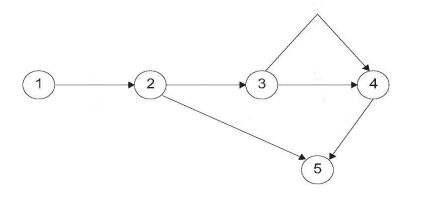
\includegraphics[width=0.5\paperwidth]{C:/Users/Admin/Desktop/Github/question_bank/LyX/static/img/9597-PJC-2016-P2-Q1-1}
\par\end{center}
\begin{enumerate}
\item Complete the PERT chart by writing the stage (A, B, \dots ) and duration
between the nodes. \hfill{}{[}4{]}
\item State the critical path. \hfill{}{[}1{]}
\item State the minimum time in which the project could be completed. \hfill{}{[}1{]}
\item For activity D: 
\begin{enumerate}
\item[(iv.1)]  state the earliest start time. \hfill{}{[}1{]}
\item[(iv.2)]  state the latest finish time. \hfill{}{[}1{]}
\end{enumerate}
\item Two stages start and end at the same nodes. Re-draw the PERT chart
by using an extra dummy stage separating them. Explain the nature
and purpose of a dummy stage. \hfill{}{[}2{]}
\item Explain dependent stages and concurrent stages. For each type of stage
give an example from this chart. \hfill{}{[}4{]}
\item Draw a Gantt chart showing all stages and their dependencies.\hfill{}
{[}4{]}
\end{enumerate}
\item Describe any \textbf{three} key stages (System analysis, System design,
System development, Testing, Implementation of computer system, Documentation,
Maintenance) of the software development life cycle. \hfill{}{[}6{]}
\item Explain why the problem must be defined accurately before the analyst
starts work. \hfill{}{[}2{]}
\item Name two methods the analyst could use to gather information about
the existing manual system. Explain how each method would be used
to gather information about this manual system. \hfill{}{[}4{]}
\item When the receptionist types an appointment for a patient, explain
why the patient name and first line of address need to be entered.
\hfill{}{[}2{]}
\item The following pseudocode algorithm describes one method of finding
an arbitrary patient name in an alphabetically ordered array of \texttt{N}
unique names. 

\noindent\begin{minipage}[t]{1\columnwidth}%
\texttt{SET first to 1 }

\texttt{SET last to N }

\texttt{REPEAT }

\texttt{\qquad{}SET mid to the integer part of (first + last)/2 }

\texttt{\qquad{}IF the mid name precedes the wanted name }

\texttt{\qquad{}\qquad{}THEN SET first to mid + 1 }

\texttt{\qquad{}ELSE }

\texttt{\qquad{}\qquad{}SET last to mid \textendash{} 1 }

\texttt{\qquad{}ENDIF }

\texttt{UNTIL first > last OR mid name is the wanted name }%
\end{minipage}
\begin{enumerate}
\item If 142 patients\textquoteright{} names are stored in the array, and
Natasha is the 44th name, state the elements of the array that are
examined when searching for Natasha.\hfill{} {[}2{]}
\item If a search is made for a name that is not in the array, what is the
largest number of elements that might need to be examined before one
could say that the name is not present? Explain how you arrive at
your answer. \hfill{}{[}2{]}
\end{enumerate}
\item Before releasing the software, it is tested using a variety of strategies.
Describe the following test strategies:
\begin{enumerate}
\item White box testing \hfill{}{[}2{]}
\item Black box testing\hfill{} {[}2{]}
\end{enumerate}
\end{enumerate}